
In addition to the simulation study, we also modelled the behaviour of eleven resident killer whales off the coast of British Columbia, Canada. The data we use were collected in August and September of 2020 and consist of tri-axial acceleration over time. Observations were collected at a rate of 50 Hz using a CATS biologger (Customizable Animal Tracking Solutions, {\em{www.cats.is}}).

%Acceleration was measured in three dimensions, which together represent the complete range of movement of an animal (forward/backward, upward/downward, and right/left). Tri-axial acceleration readings are common in these types of tags and are often used to infer animal behaviour such as foraging \citep{Fehlmann:2017,Wright:2017,Cade:2017}. The act of attaching and detaching the tag caused anomalous behaviour before 1:20 p.m. and after 6:00 p.m., so observations taken during these time periods are ignored. There were also periods of time when the tag failed to record observations, resulting in data gaps between 2:25 p.m. and 2:37 p.m. and between 4:07 p.m. and 5:07 p.m. 

We divide the accelerometer data into two-second windows, each consisting of 100 accelerometer readings. We then perform a Fourier transform within each two-second window, and summarize the window with two measures of ``wiggliness":
(1) the sum of the squares of all Fourier coefficients corresponding to frequencies less than 5 Hz, and (2) the sum of the squares of all Fourier coefficients corresponding to frequencies greater than 5 Hz. We use a hierarchical hidden Markov model \citep{Barajas:2017} to test our algorithm on complicated models, and fine-scale biologging data often exhibits multi-scale behaviour \citep{Sidrow:2021}. We select a total of $N_c = 3$ coarse-scale states and $N_f^{(i)} = N_f = 3$ fine-scale states for each coarse-scale state. However, we enforce that the state-dependent fine-scale distributions are shared across coarse-scale states. In practice, the number of hidden states in a Hidden Markov model should be selected using model selection and validation techniques as well as with the help of subject-matter experts \citep{Pohle:2017}. However, we select $N_c = 3$ and $N_f = 3$ to be in line with common values in the statistical ecology literature. The preprocessed data contain a total of $T=89462$ two-second windows. We have plotted the data corresponding to one of the whales in Figure (\ref{fig:data}). The depth and wiggliness data are colour-coded by the most likely coarse- and fine-scale hidden states conditioned on the MLE parameters.
%
\begin{figure}
    \centering
    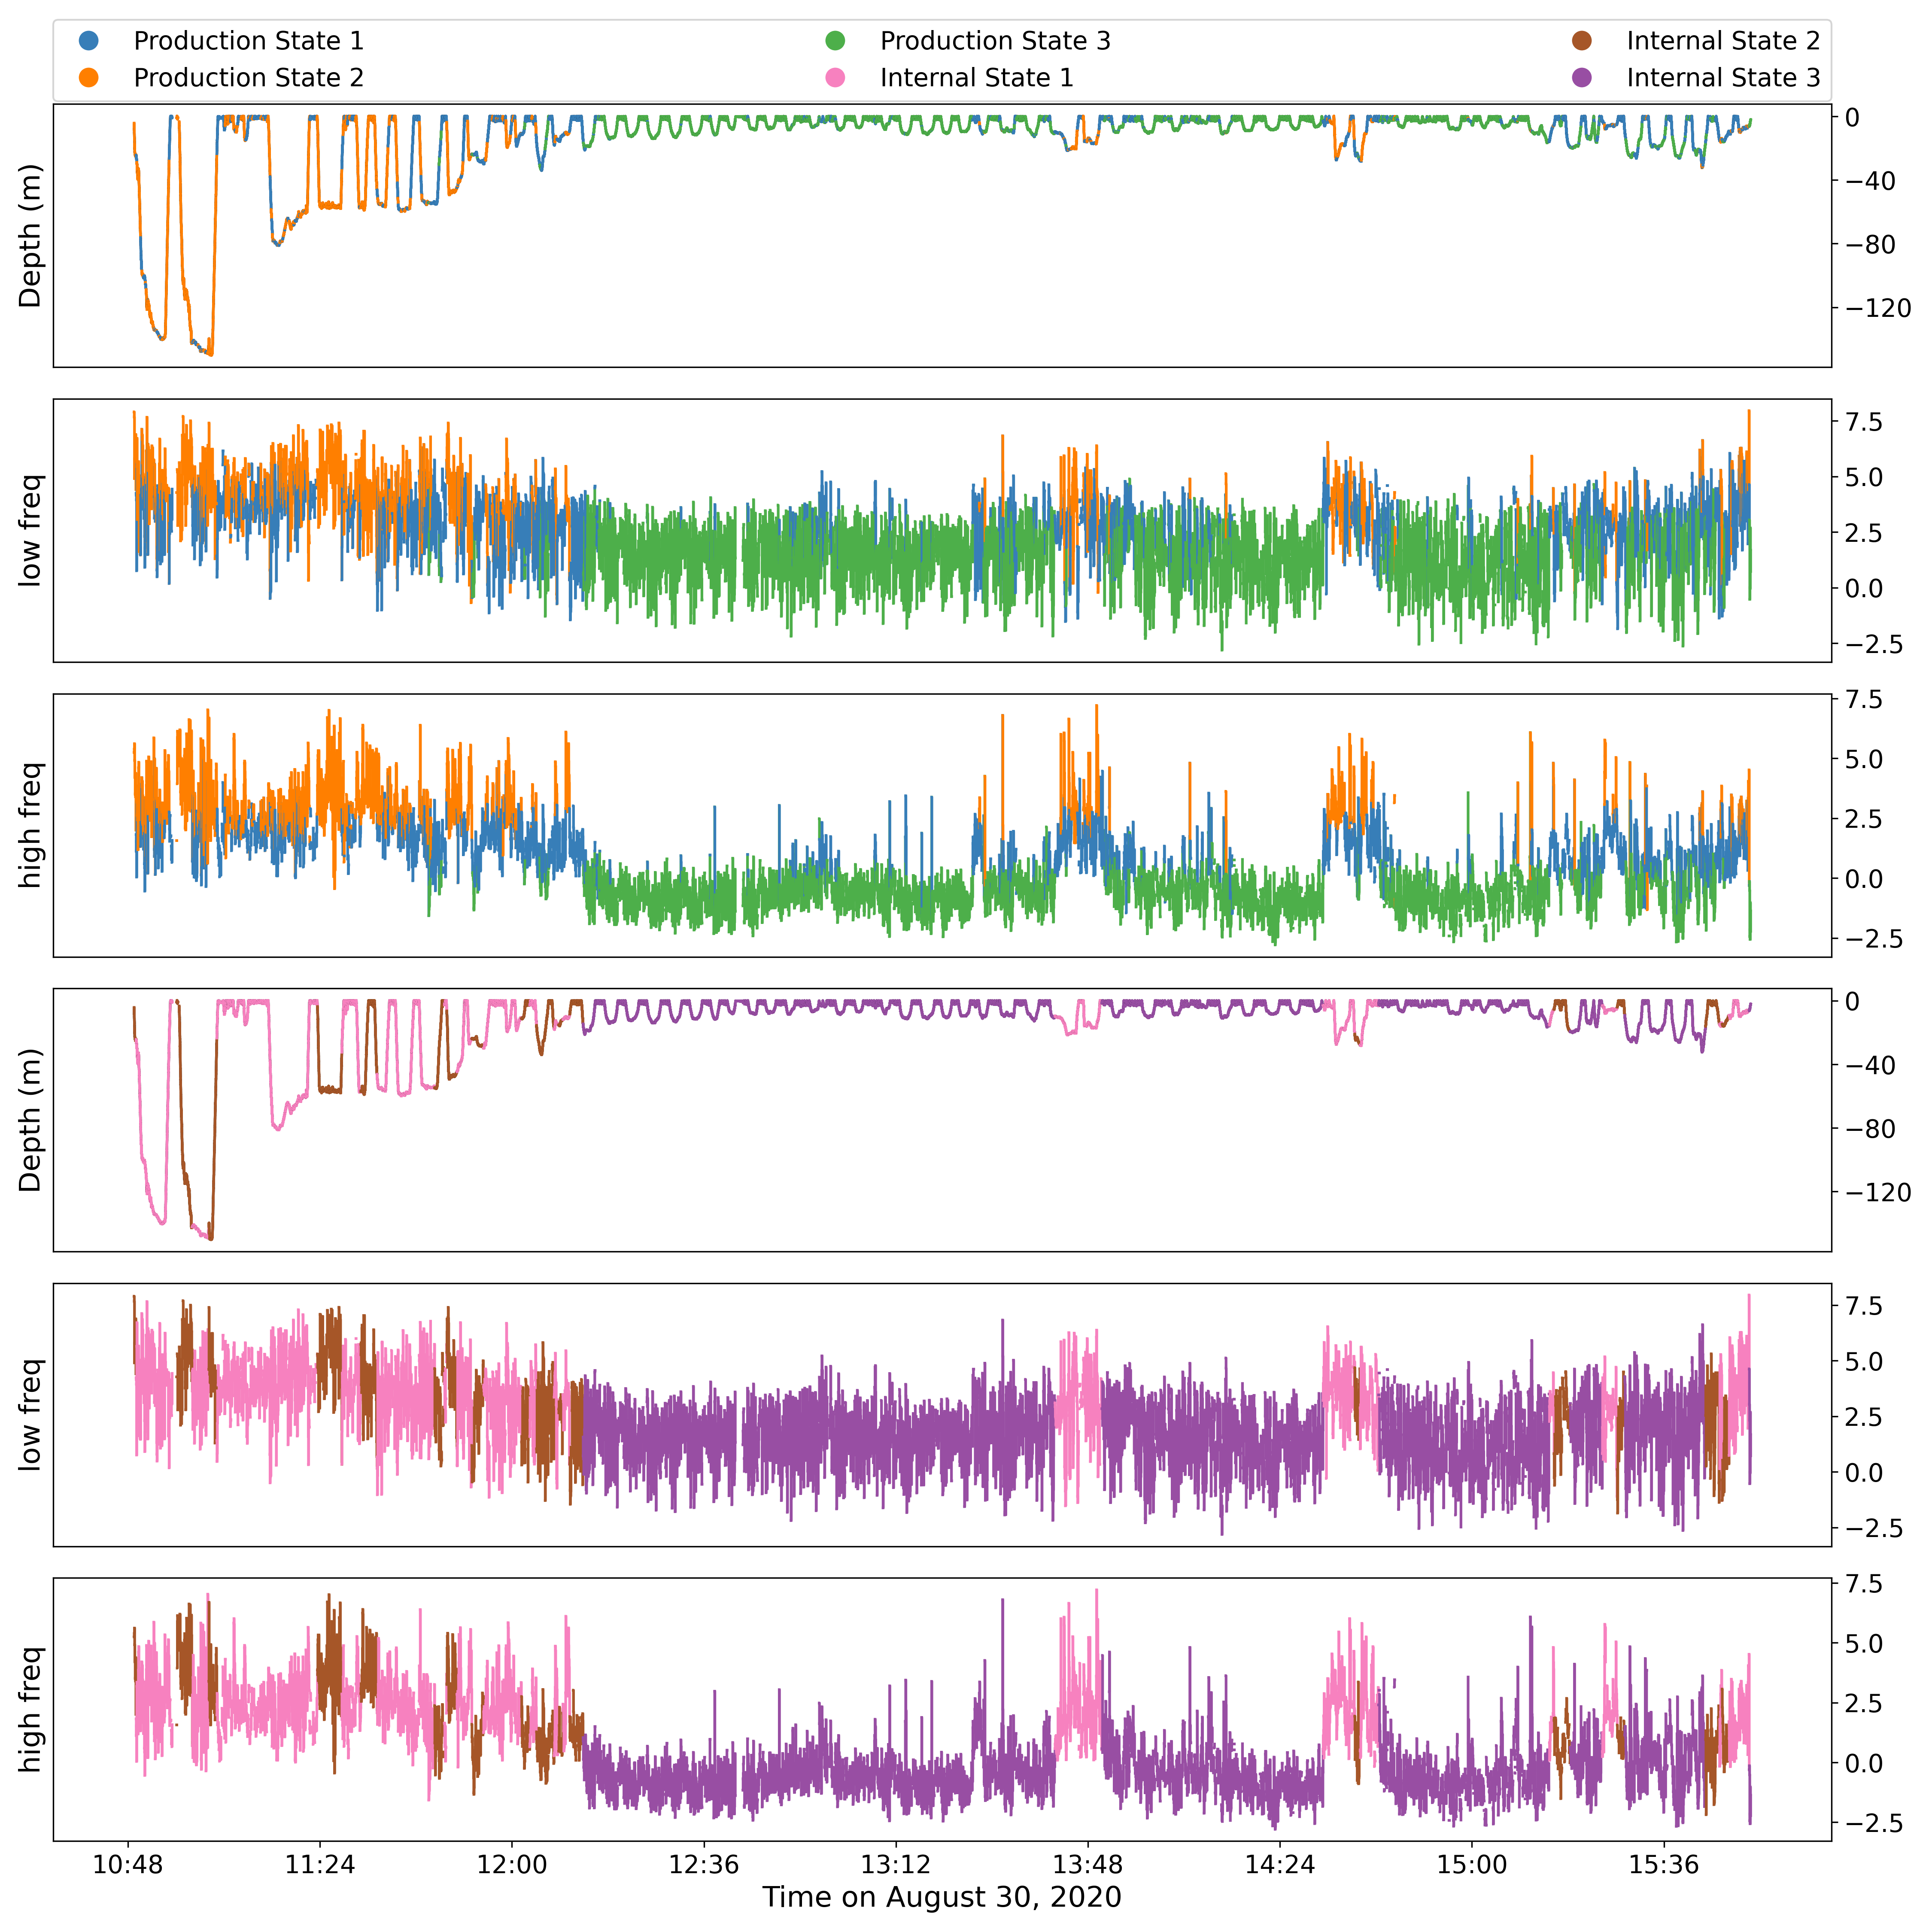
\includegraphics[width=6.5in]{plt/decoded_dives_kw_I145_K_3_3_nWhales_8.png}
    \caption{Dive profile and ``wiggliness" associated with a selected Killer Whale off the coast of British Columbia, Canada. Data is colour-coded according to the most likely hidden coarse-scale and fine-scale state of each two-second window.}
    \label{fig:data}
\end{figure}
%
Production states 3, 1, and 2 appear to correspond to increasing activity, respectively. Internal states 1 and 2 appear to correspond to varying level of activity when the killer whale is hunting, while internal state 3 appears to correspond to resting behaviour.

We used a similar procedure to the simulation study to initialize the HMM parameters. In particular, let $\bar y$ and $\bfQ$ denote the sample mean and sample covariance of $\{y_t\}_{t=1}^T$, respectively. For inference, we initialized $\theta_0$ as
%
\begin{equation*}
    \mu^{(i)}_0 \sim \calN(\bar y, \text{diag}(\bfQ)), \quad \Sigma^{(i)}_0 = \text{diag}(\bfQ), \qquad i \in \{1,\ldots,N_f\},
\end{equation*}
%
Note that we only define emission distributions for $i = 1,\ldots,N_f$ because we assume that each coarse-scale state has the same fine-scale emission distributions.
Throughout the optimization procedure, we assume that $\Sigma^{(i)}$ is diagonal for all $i \in \{1,\ldots,N_f\}$.
%
We initialized $\eta_{c,0}$ as
%
\begin{align*}
    \eta^{(i)}_{c,0} &\sim \calN(0,1), & i & = 2,\ldots,N_c \\
    %
    \eta^{(i,j)}_{c,0} &\sim \calN(-2,2^2), & i,j & = 1,\ldots,N_c, \qquad i \neq j.
\end{align*}
%
We initialized all elements of $\eta_{f,0}$ corresponding to the fine-scale initial distributions $\delta^{(i)}_f \in \bbR^{N_f}, i = 1,\ldots,N_c$ with a standard normal distribution, i.e. $\calN(0,1)$. We initialized all elements of $\eta_{f,0}$ corresponding to the fine-scale transition probability matrices, $\mathbf{\Gamma}^{(i)}_f \in {\bbR^{N_f \times N_f}}, i = 1,\ldots,N_c$ with a normal distribution centred at -1 with variance 1, i.e. $\calN(-1,1)$.

%If the 2-norm of the average estimated gradient $||\frac{1}{T}\sum_{t=1}^T \widehat \nabla F^{(k,m)}_t + \widehat \nabla G^{(k,m)}_t||$ ever fell below a tolerance of $10^{-8}$, we terminated the M-step of algorithm and moved on to the E-step. Likewise, if the relative change of the log-likelihood after one full E- and M- step of the EM algorithm ever fell below a tolerance of $10^{-10}$, we terminated the algorithm altogether. We found the ground truth MLEs by running the traditional EM algorithm until the relative change in the log-likelihood was on the order of machine precision $10^{-15}$.

We estimated the parameters of the hierarchical HMM for this case study the same six new inference algorithms and three baseline algorithms from the simulation study.
%
All algorithms were run using 50 random initializations for a total of 12 hours each on Compute Canada Cedar nodes with 16GB of RAM.
%
Figure (\ref{fig:ll_trace_case}) displays the log-likelihood (divided by $T$) of the MLE minus the log-likelihood (divided by $T$) at each epoch. For each optimization algorithm we present the random initialization that resulted in the highest likelihood after 12 hours of computation.
%
\begin{figure}
    \centering
    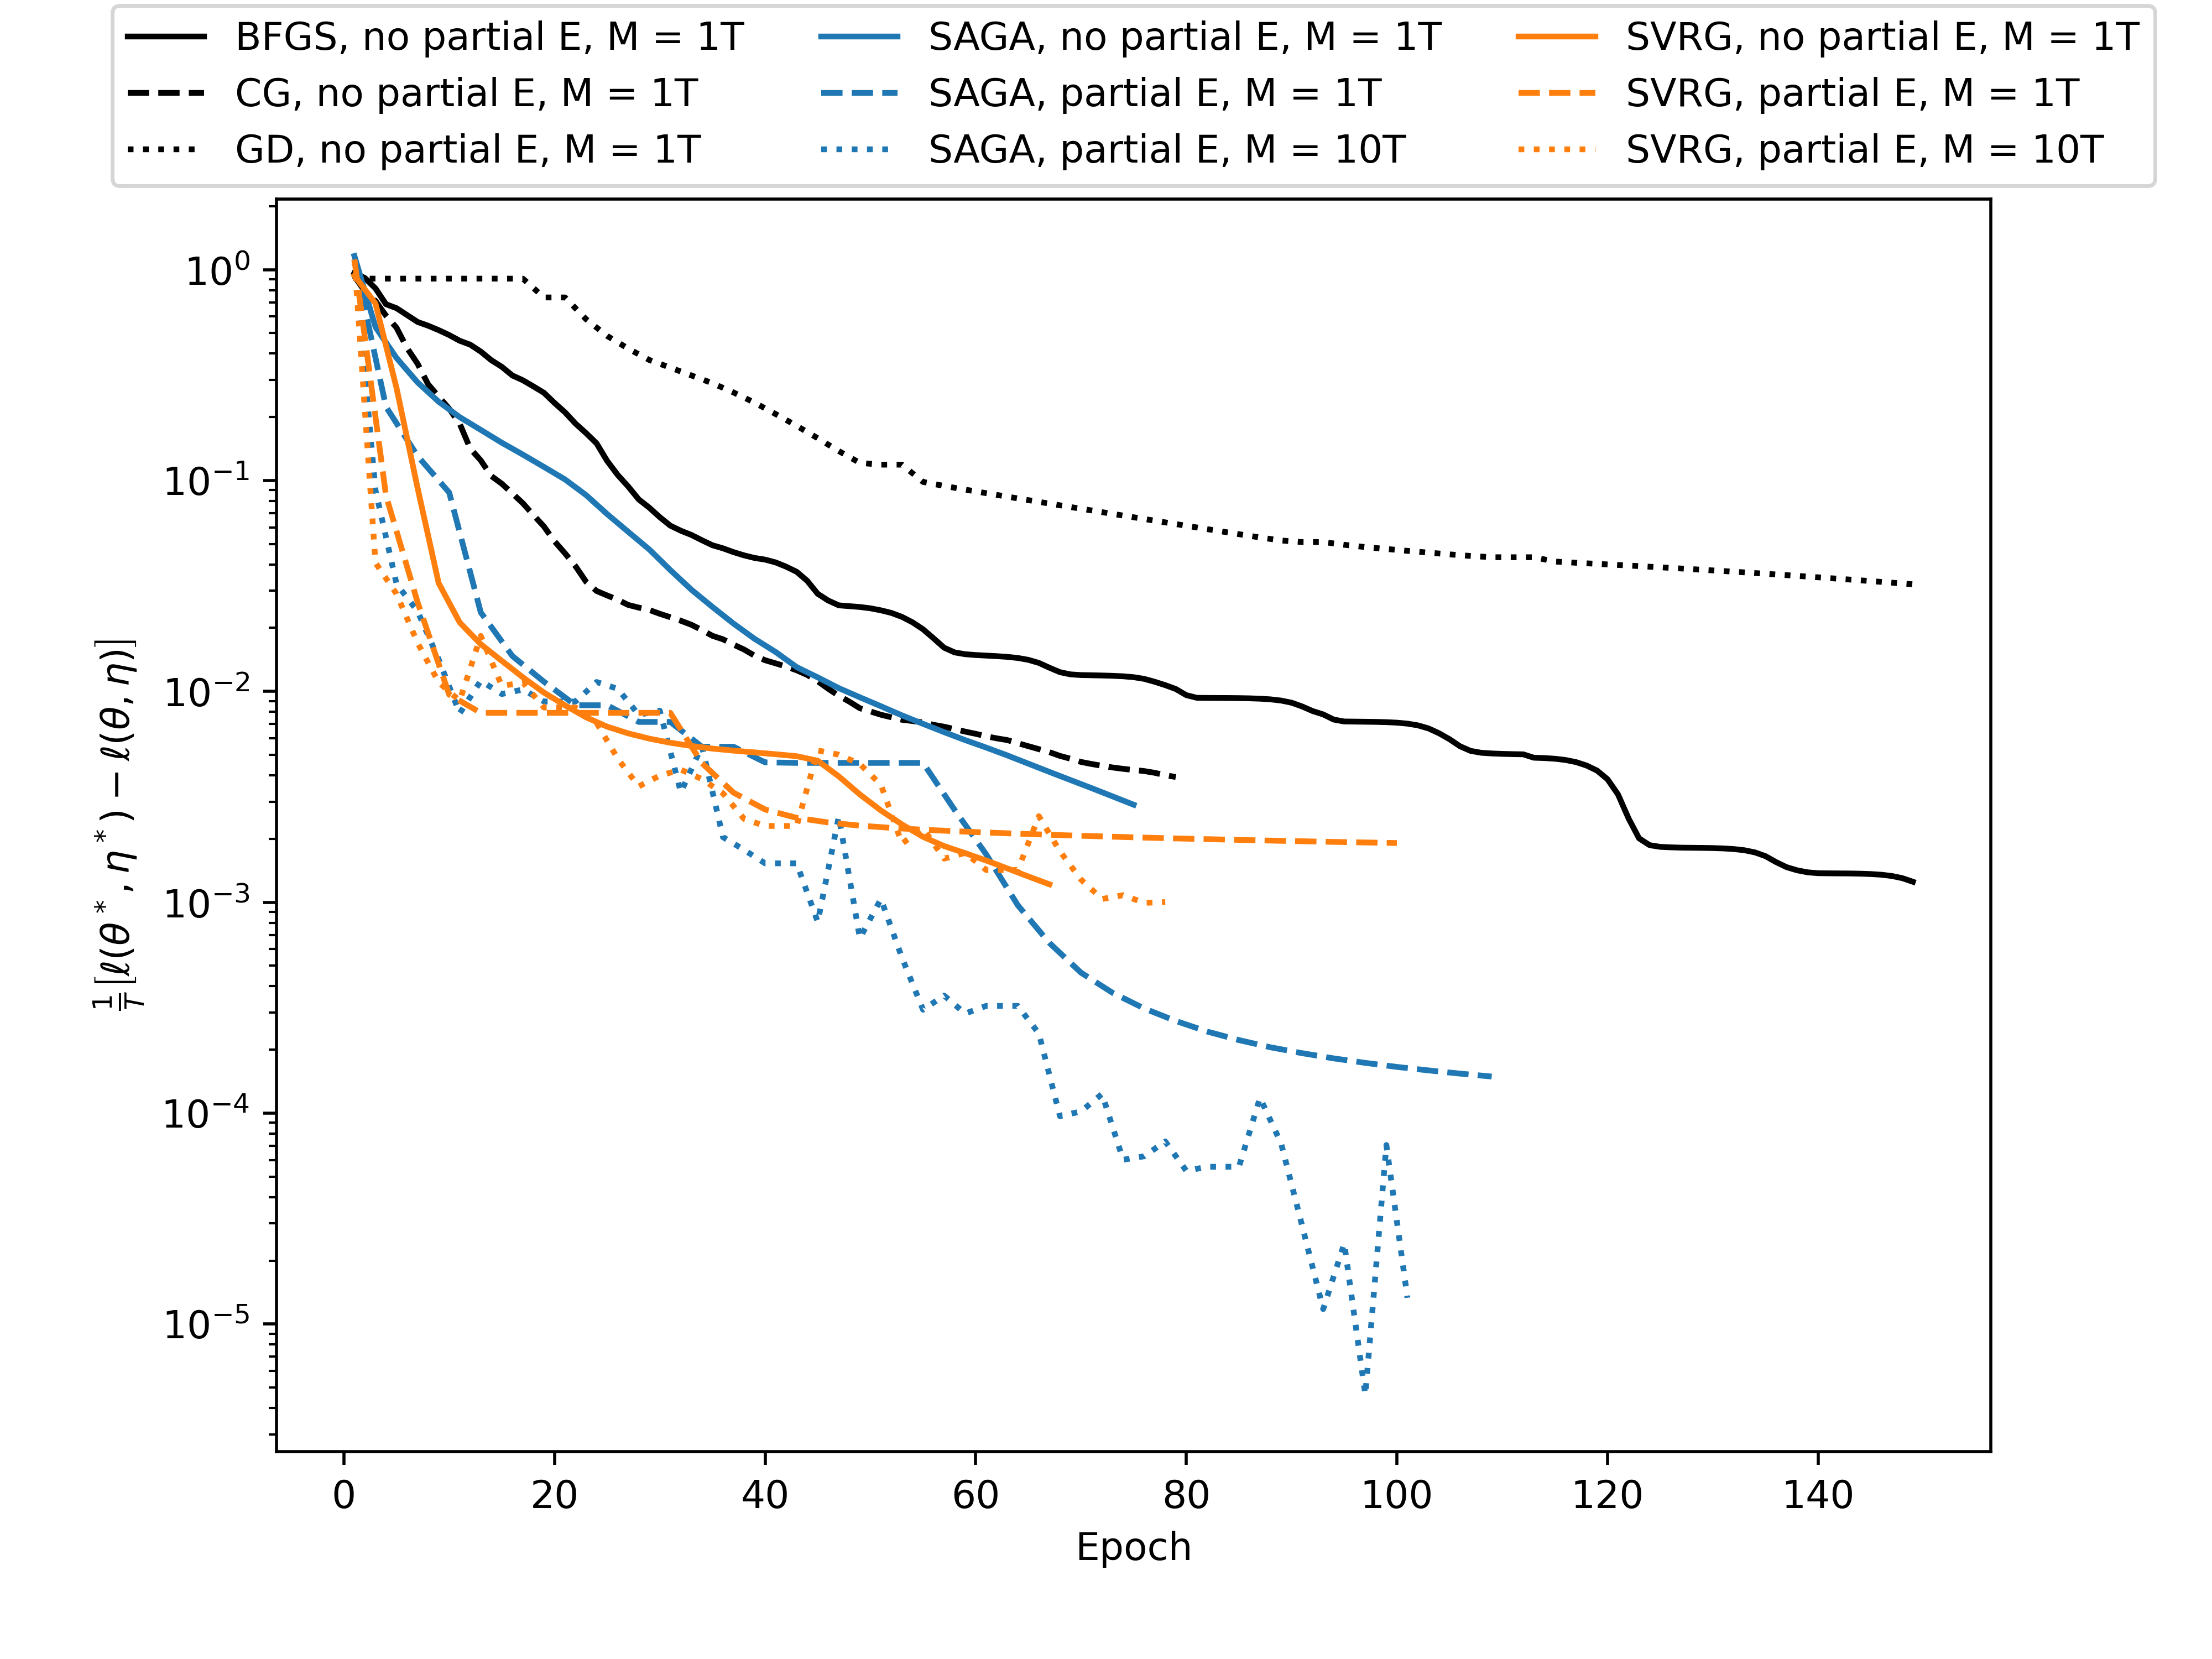
\includegraphics[width=6in]{../plt/log-like_v_epoch_K-3-3.png}
    \caption{Optimally gap between the log-likelihood and optimal log-likelihood for the estimated parameters of the HMM from the Killer Whale case study. One epoch represents either one full E-step, $T$ iterations with the M-step, or one gradient step for full-gradient algorithms. The y-axis is on a log-scale.}
    \label{fig:ll_trace_case}
\end{figure}
%
Figure (\ref{fig:boxplots_case}) shows box plots of both the number of epochs until convergence as well as the optimality gap (log likelihood divided by $T$) at convergence for each algorithm. Convergence is defined as the point at which the gradient norm of the log-likelihood (divided by $T$) was less than $10^{-2}$.
%
\begin{figure}
    \centering
    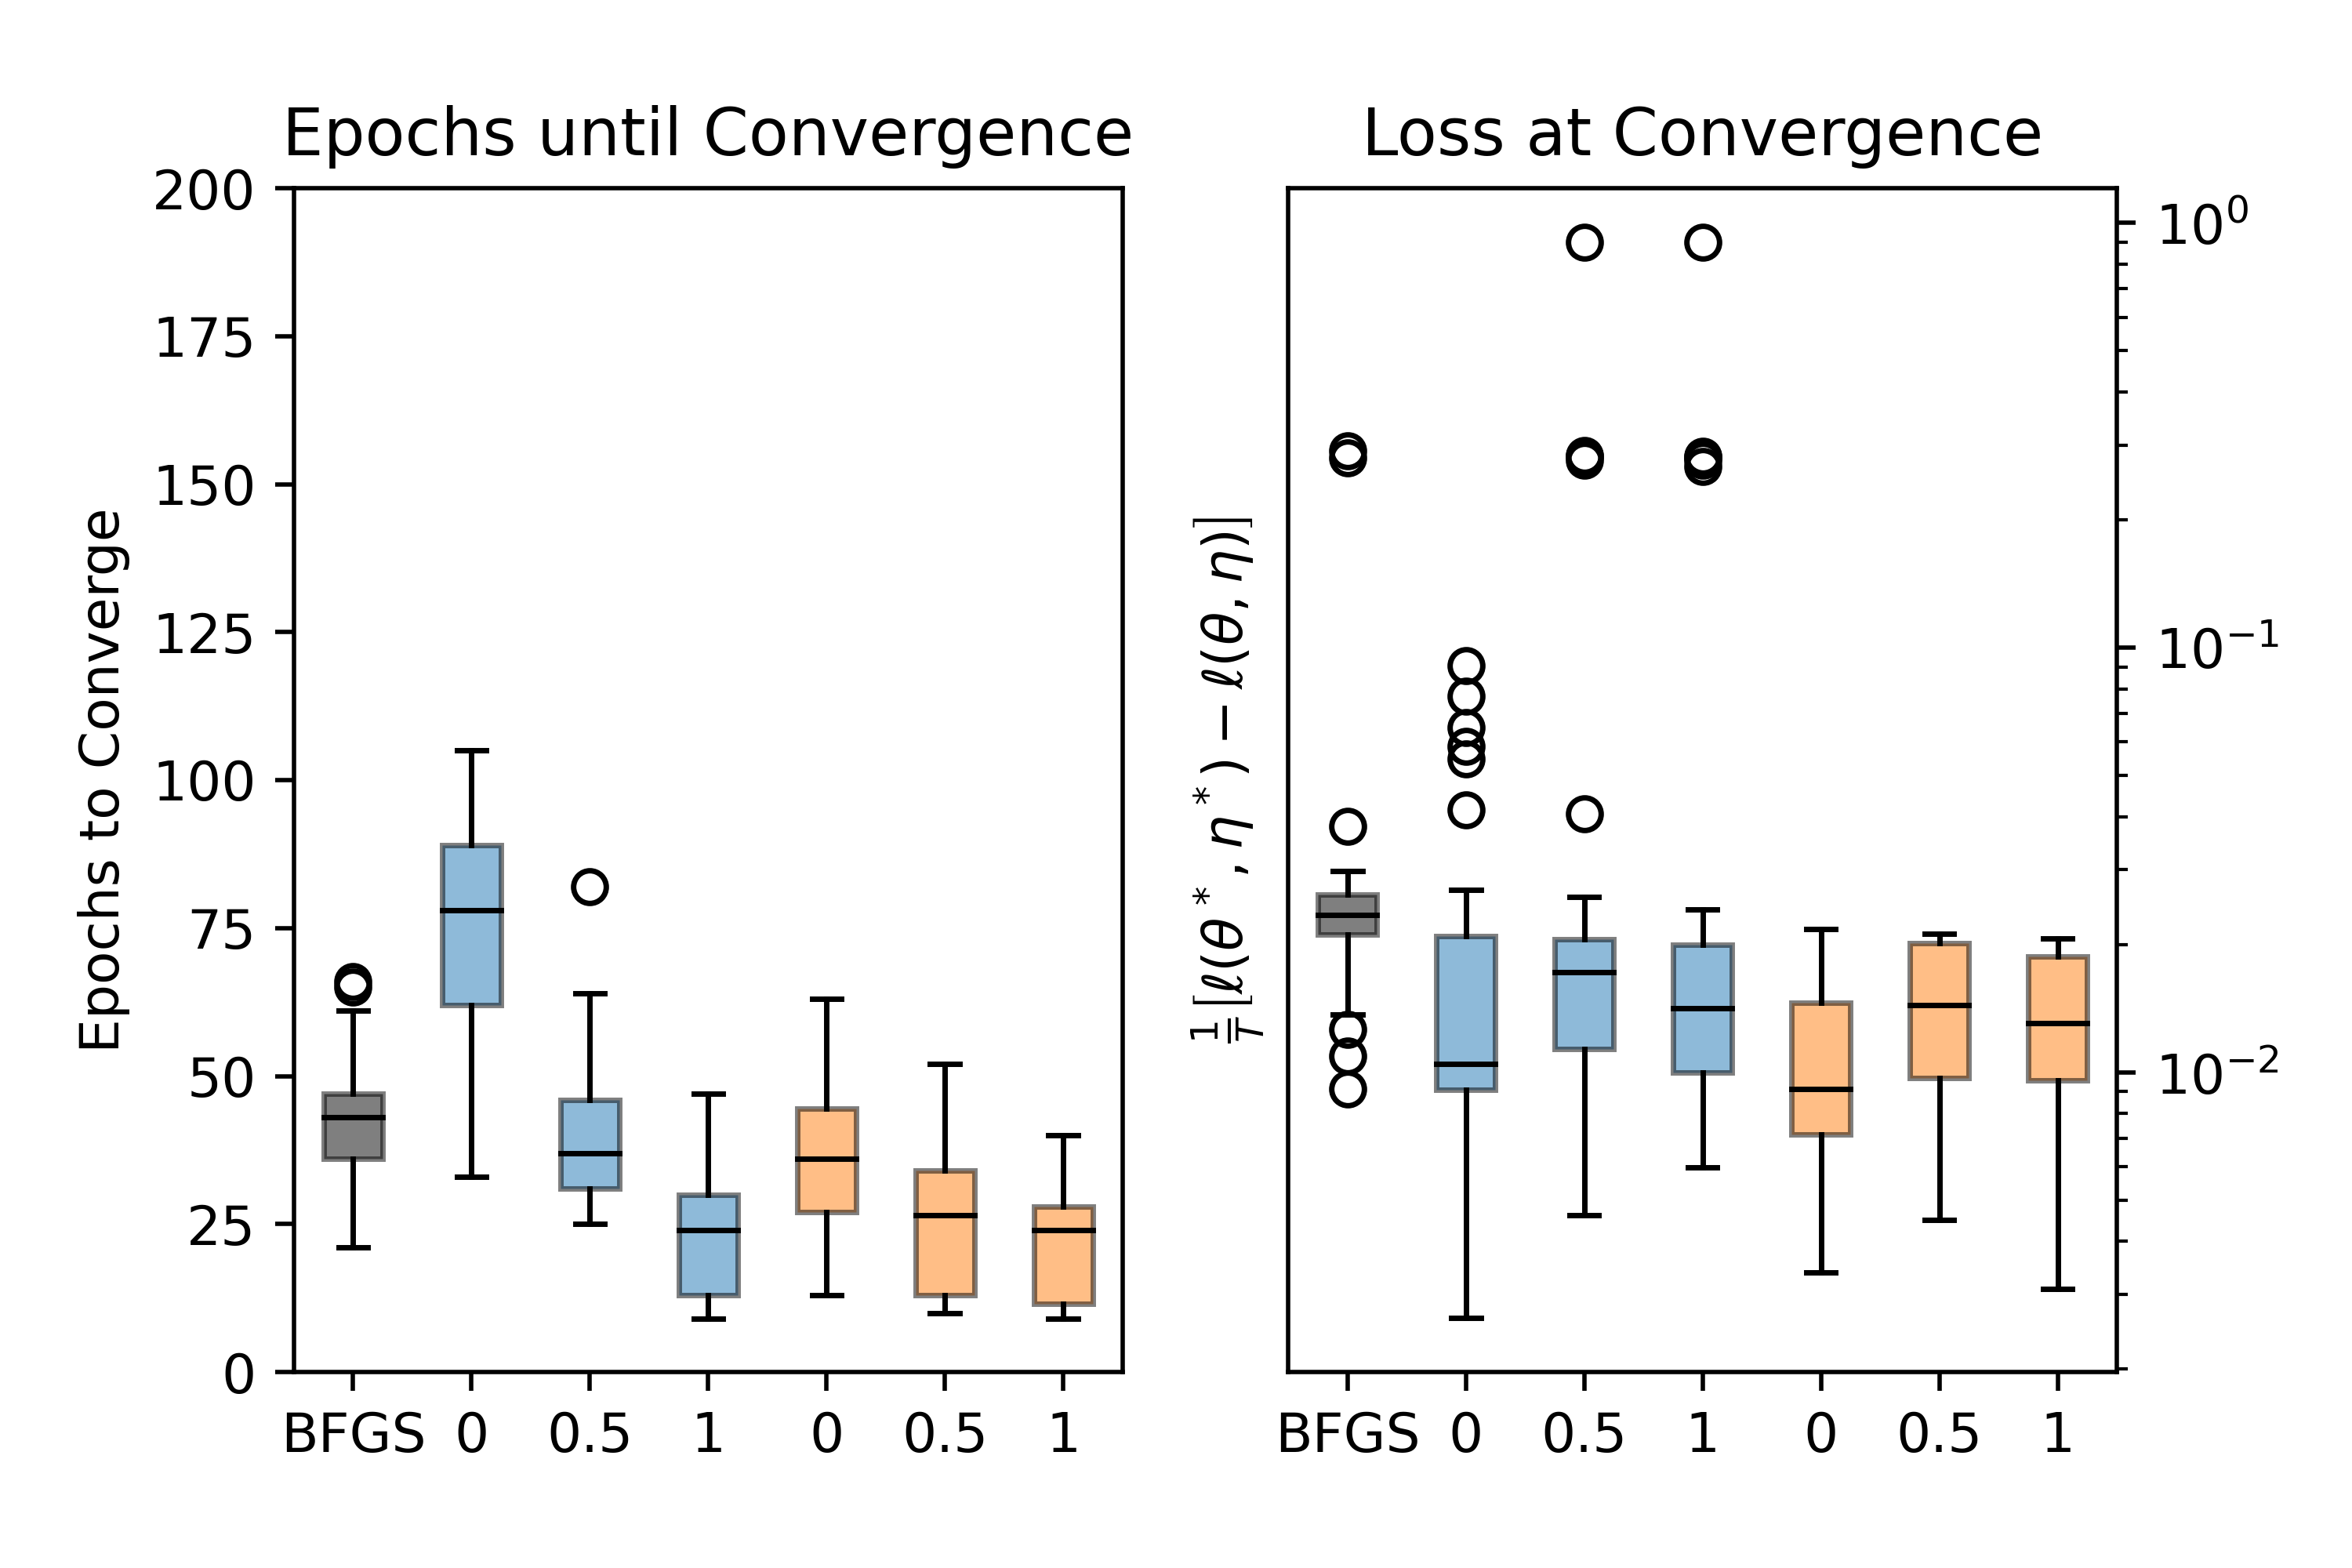
\includegraphics[width=6.5in]{../plt/boxplots_case_study.png}
    \caption{Box plots showing Epochs to converge and the optimality gap at convergence for each optimization algorithm. NPE corresponds to no partial E step, PE1 corresponds to a partial E step with $M=T$, and PE2 corresponds to a partial E-step with $M=10T$. Blue corresponds to SAGA and orange corresponds to SVRG.}
    \label{fig:boxplots_case}
\end{figure}
%
All new algorithms converge to regions of lower loss on average, and all algorithms except for SAGA without a partial E-step converge in fewer epochs than BFGS.
%
Figure (\ref{fig:scatter_case}) displays scatter-plots of the number of epochs to converge and the loss at convergence of each algorithm vs. BFGS for the same data set and parameter initialization. For each 
%
\begin{figure}
    \centering
    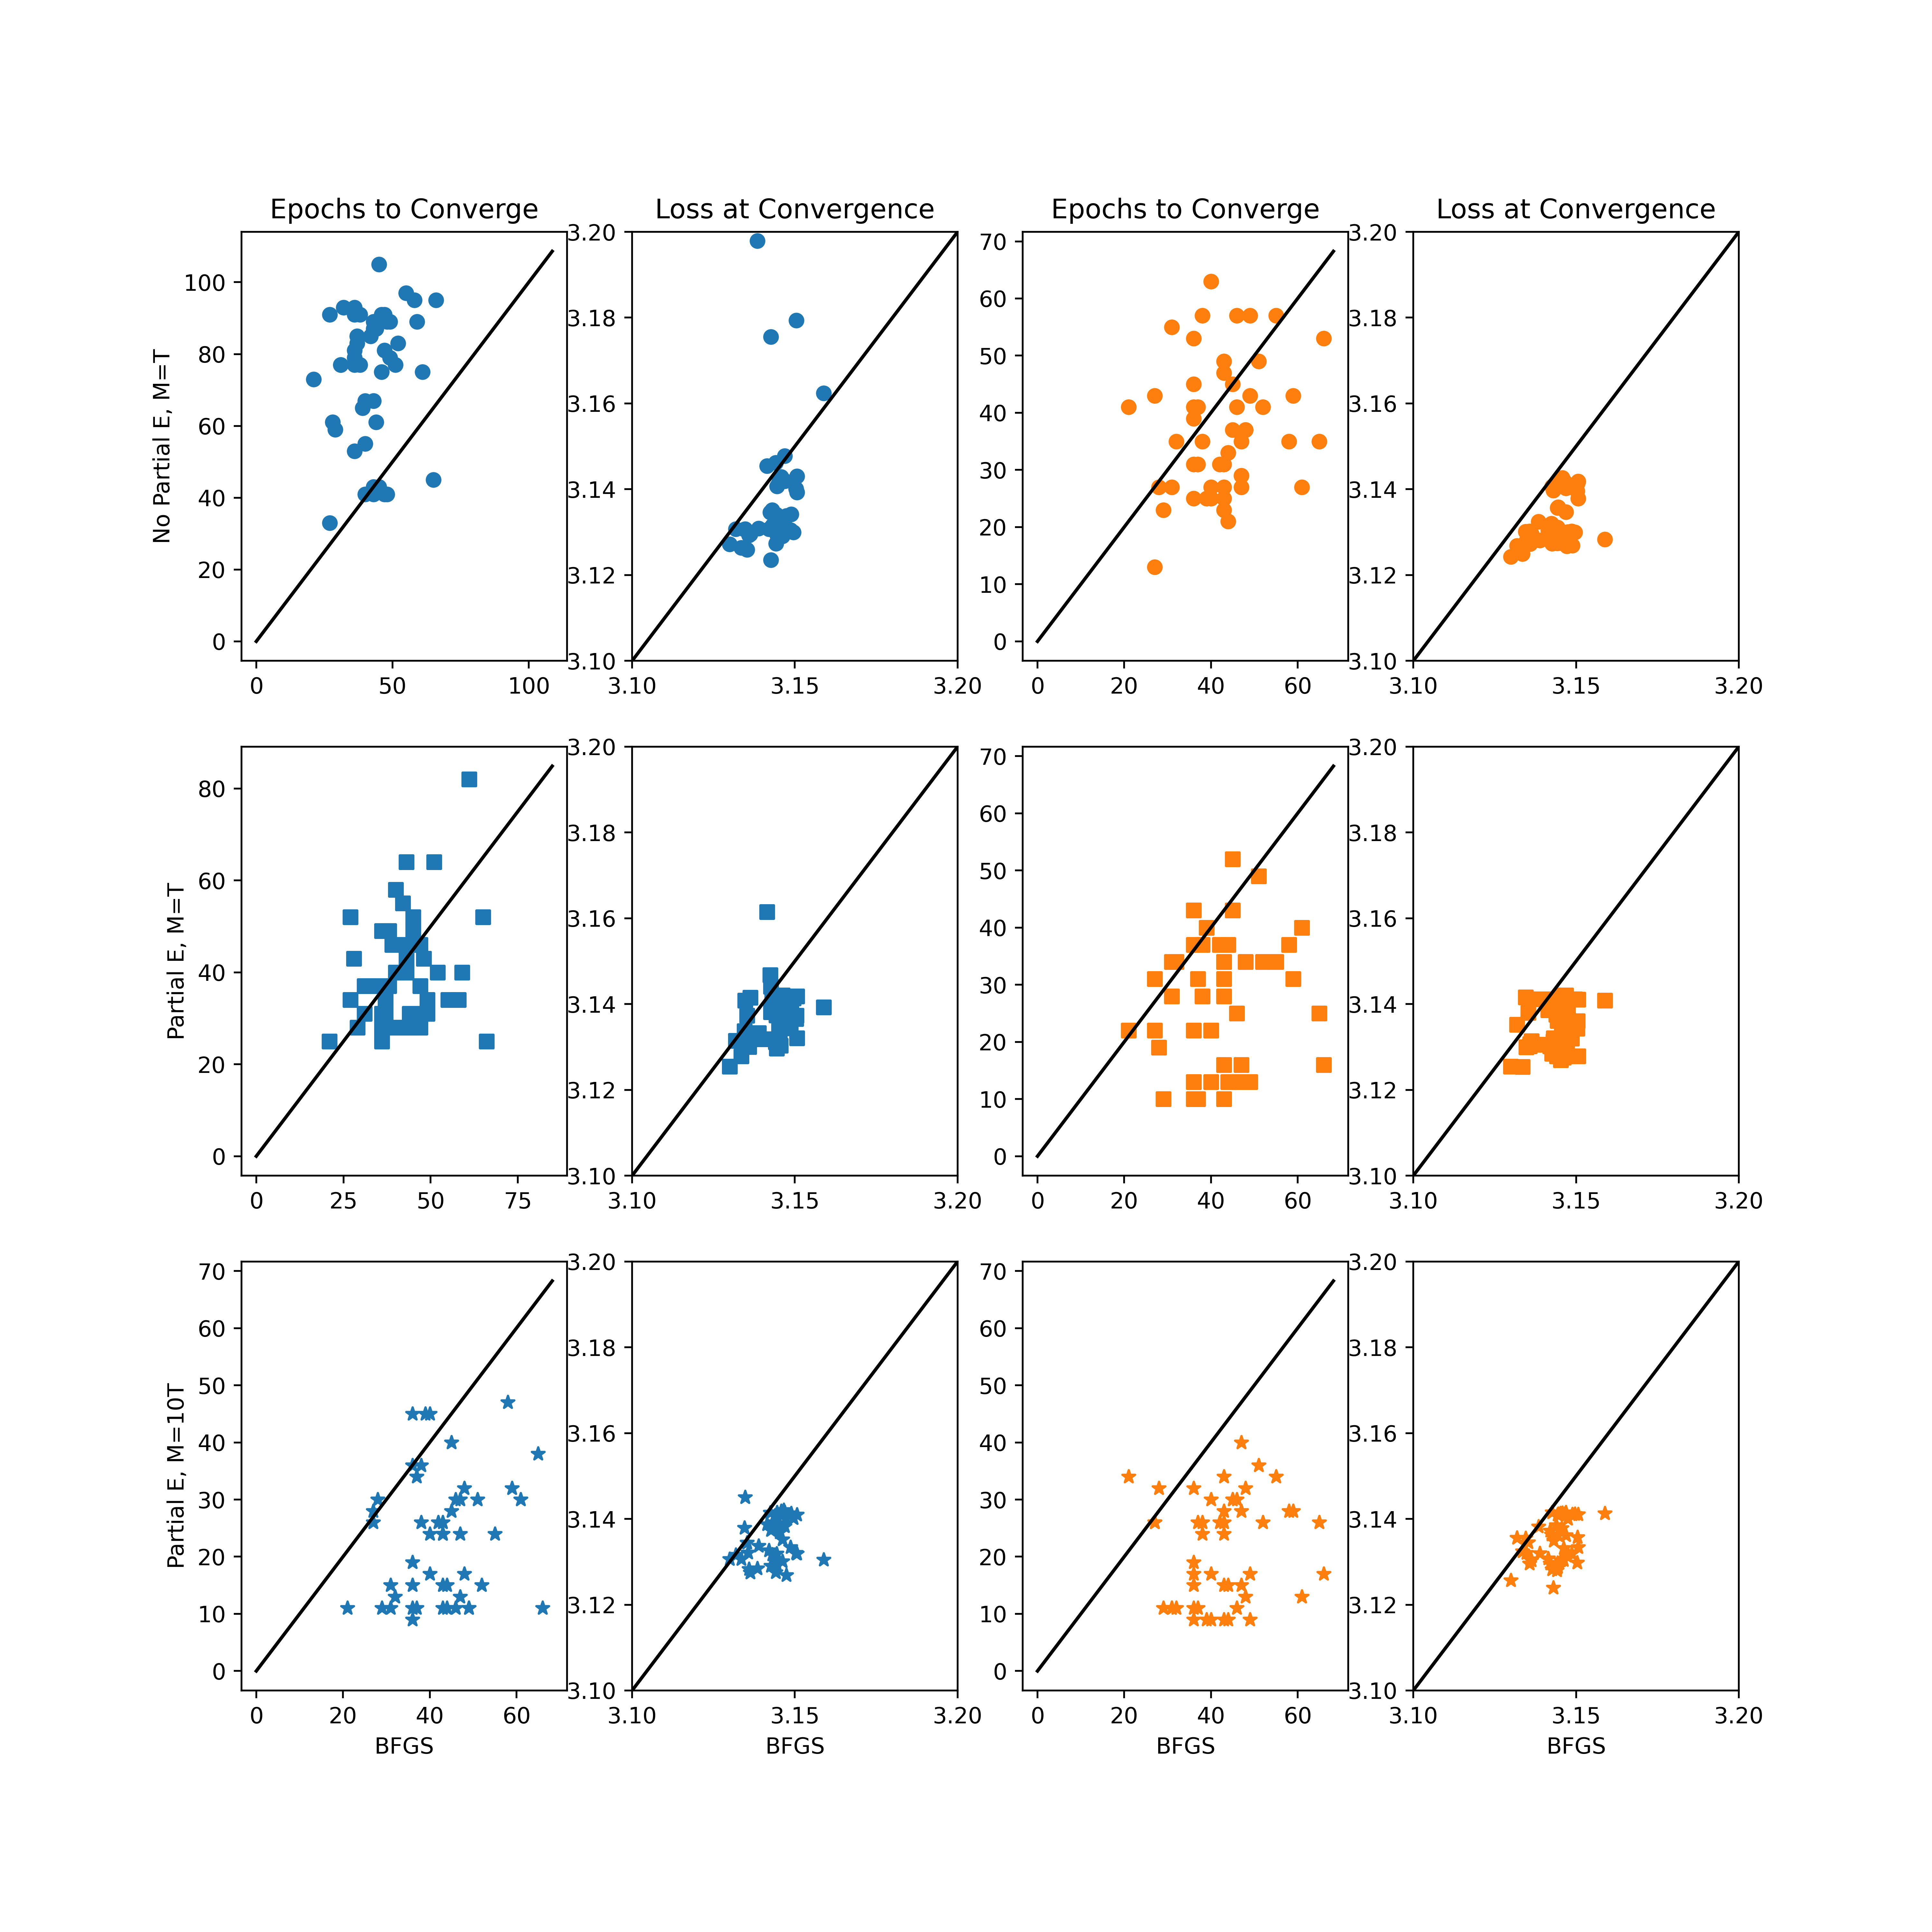
\includegraphics[width=6.5in]{../plt/paired_scatter_case_study.png}
    \caption{number of epochs to converge (columns 1 and 3) and the loss at convergence (columns 2 and 4) of each algorithm vs. BFGS for identical same data sets and parameter initializations. Lower is better for both criteria, so data points below the line $y=x$ suggest that the stochastic optimization algorithms perform better.}
    \label{fig:scatter_case}
\end{figure}
%
Like the simulation study, SVRG appears to converge faster than SAGA for all algorithms. This may be a function of our step size ($1/3 \hat L$), but that step size was selected based upon suggestions from the SAGA paper \citep{Defazio:2014}. In addition, SVRG converges faster than the baseline when using a partial E-step, and SAGA converged faster than the baseline with a partial E step and $M=10T$. All stochastic optimization algorithms tend to converge to areas of lower loss than BFGS. 

%SAGA without a partial E-step performs similarly to the EM algorithm in a per-epoch basis because SAGA is successfully converging for the M-step when $M = T$. However, it does not perform as well as the EM algorithm on a per-time basis because the M-step is significantly slower when using SAGA vs the closed-form solution. This behaviour is expected, and SAGA has a significant advantage over the EM algorithm in that it only requires gradients rather than sufficient statistics.

%mplementing a partial E-step shows that SAGA can outperform the EM algorithm when the parameter estimates are far from the optimal solutions and when the underlying HMM does not mix rapidly. This is likely because the weights of the $F$ and $G$ are very inaccurate at first, and updating them early in the optimization procedure yields a significant speed-up. In addition, if the Markov chain is rapidly mixing, then updates to $\gamma_{t_m}$ and $\xi_{t_m}$ at a single data point are more accurate. Future work may involve performing the partial-E step for many weights at once sequentially, depending upon the mixing time of the current estimate of $\eta_k$.